%%% Local Variables:
%%% mode: latex
%%% TeX-master: "../index"
%%% End:

% Recommended:
% Show symmetric-key example with Alice-Bob diagram
% Mention modern algorithm (e.g. AES, Triple-DES)
% Benefits of public-key encryption (no key sharing)
% Show public-key example with RSA and Alice-Bob diagram

\subsection{Agenda}
\begin{enumerate}
\item Symmetric-key encryption
\item Symmetric- vs. public-key encryption
\item RSA
\end{enumerate}

\subsection{Symmetric-key encryption}
\subsubsection{Set up}
\begin{itemize}
  \item $m \in \mathcal{P}$ is the plaintext
  \item $k \in \mathcal{K}$ is the key
  \item $c \in \mathcal{C}$ is the ciphertext
  \item $e_k(m)$ encryption function
  \item $d_k(c)$ decryption function
\end{itemize}

\begin{figure}[H]
  \begin{centering}
    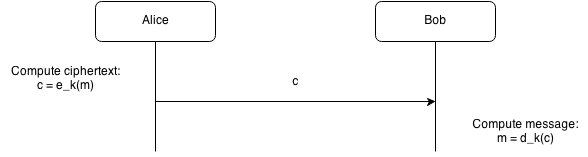
\includegraphics[width=15cm]{images/1-sym-enc}
    \caption{Basic model for symmetric encryption}
  \end{centering}
  \label{fig:sym-enc}
\end{figure}

\subsubsection{Modern implementations}
\begin{description}
\item[DES] 64-bit block cipher with 56-bit key. Due to small key,
  exhaustive search is a possibility. Therefore, \emph{Triple-DES} was
  made.
\item[AES] 128-bit block cipher with 128 to 256-bit key.
\end{description}

\subsection{Symmetric- vs. public-key encryption}
\begin{description}
\item[Pros] Faster and easier to implement
\item[Cons] Requires both parties can access the secret key. Impossible?
\end{description}

\subsection{RSA}
